\documentclass[12pt, a4paper]{article}
\usepackage[utf8]{inputenc}
\usepackage[russian]{babel}
\usepackage[pdftex]{graphicx, color}
\usepackage{amsmath}
\usepackage{amsfonts}
\usepackage{amssymb}
\usepackage{amsthm}
\usepackage[left=2cm,right=1.5cm,top=1.5cm,bottom=2cm]{geometry}
\usepackage{indentfirst}
\usepackage{hyperref}

\usepackage{setspace}
\onehalfspacing
\graphicspath{{pic/}}

\begin{document}

	\thispagestyle{empty}

	\begin{singlespace}
	\begin{titlepage}
		\begin{center}
			
\includegraphics[height = 3cm]{msu.png}

			{\scshape Московский государственный университет имени М.~В.~Ломоносова}\\
			Факультет вычислительной математики и кибернетики\\
			\centerline{\hfill\hrulefill\hrulefill\hrulefill\hrulefill\hfill}

			\vfill

			{\LARGE Отчет к третьему заданию практикума на ЭВМ: \\ Метод опорных векторов}

			\vspace{1cm}

		\end{center}

		\vfill
		\begin{flushright}
			\textit{Студент 3 курса ВМК (317 группа):}\\
				Оспанов А.М.

			\vspace{5mm}

		\end{flushright}

		\vfill

		\begin{center}
		Москва, 2014
		\end{center}
	\end{titlepage}
	\end{singlespace}

	\tableofcontents


	\newpage
	\section{Введение}
		Данный отчет написан к третьему заданию практикума на ЭВМ 317 группы. Тема задания: Метод опорных векторов. Отчет написан студентом 317 группы -- Оспановым Аятом.

		В данной работе были реализованы разные методы решения задачи SVM. Были проведены исследования по оценке времени работы методов и исследования по подбору констант и прочие исследования. Были проведены тесты применимости данных методов в реальных задачах на примере классификации MNIST.

	\newpage
	\section{Основная часть}
		\subsection{Предварительный подсчет данных для решения задач}
			{\bf Вывод формулы субградиента для функционала в прямой задаче SVM}

			Надо найти следующий субдифференциал 
			$$ \partial(\frac{1}{2} \left \| x \right \|^2 + C\sum^{n}_{n=1} {max \{0, 1 - y_n w^T x_n \}}) $$

			Для начала найдем субградиент фунцкии $$ F(x) = max \{ f_1(x), f_2(x) \} $$
			
			Субградиент для данной функции определяется следующим образом:
			
			Если $ f_1(x) > f_2(x)$, то $\partial F = \{\nabla f_1(x) \}$
			
			Если $ f_2(x) > f_1(x)$, то $\partial F = \{\nabla f_2(x) \}$
			
			Если $ f_1(x) = f_2(x)$, то $\partial F = [ min \{ \nabla f_1(x), \nabla f_2(x) \}, max \{ \nabla f_1(x), \nabla f_2(x) \} ] $

			Учитывая это, получаем
			$$ \partial (max\{ 0, 1 - y_n w^T x_n \}) = 
			\left\{
			\begin{array}{l l}
				\{0\},\ y_n w^T x_n > 1 \\
				\{-y_n x_n\},\ y_n w^T x_n < 1 \\ 
				$[$ min \{ 0, -y_n x_n \}, max \{ 0, -y_n x_n \} $]$ ,\ y_n w^T x_n = 1
			\end{array}
			\right.
			$$

			В итоге получим следующий субдифференциал
			$$ \partial \left( \frac{1}{2} \left \| x \right \|^2 + C\sum^{n}_{n=1} {max \{0, 1 - y_n w^T x_n \}} \right) = w + C\sum^{n}_{n=1} \partial (max\{ 0, 1 - y_n w^T x_n \})$$
		
		\newpage
		\subsection{Пункт 1}
			Исследуем зависимость времени работы методов от размерности пространства для каждого размера выборки в методах с линейным ядром.
			
			На слелующих фото представлены графики зависимости времени работы от размерности пространства. На них можно увидеть, что самый быстрый метод libsvm, далее liblinear

			\begin{center}
				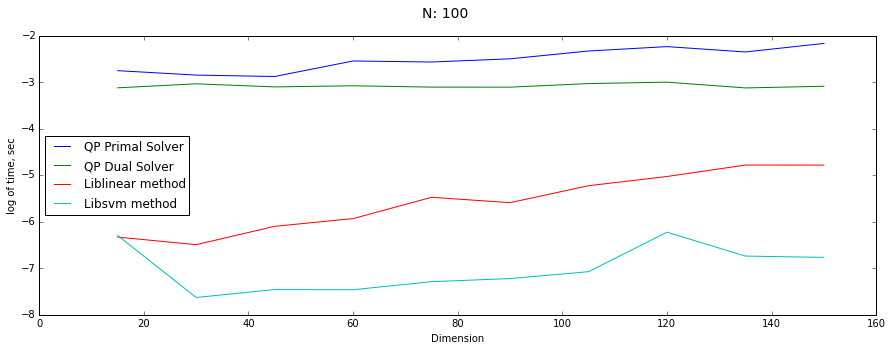
\includegraphics[width=17cm]{1par_N100_one.png}
			\end{center}

			\begin{center}
				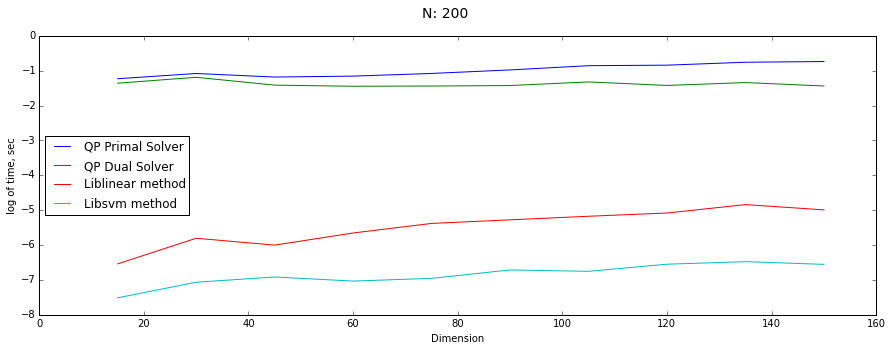
\includegraphics[width=17cm]{1par_N200_one.png}
			\end{center}

			\begin{center}
				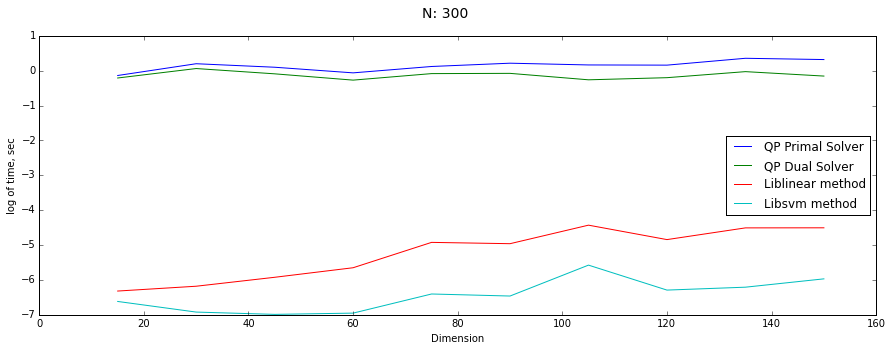
\includegraphics[width=17cm]{1par_N300_one.png}
			\end{center}

			\begin{center}
				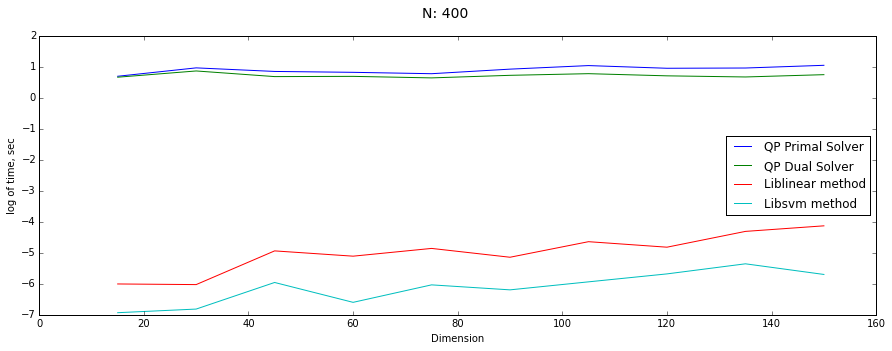
\includegraphics[width=17cm]{1par_N400_one.png}
			\end{center}

			\begin{center}
				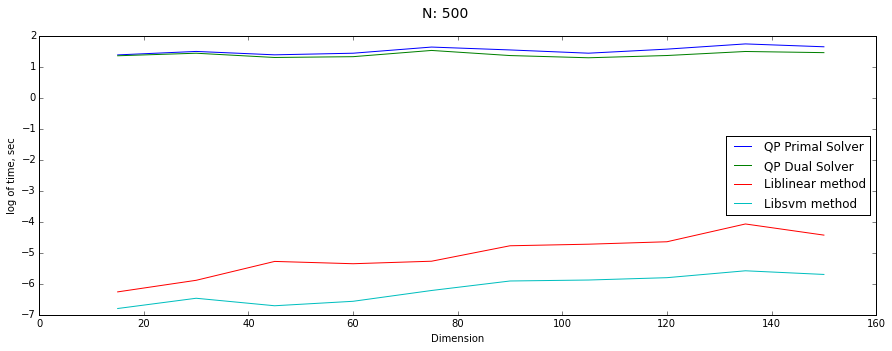
\includegraphics[width=17cm]{1par_N500_one.png}
			\end{center}

			\begin{center}
				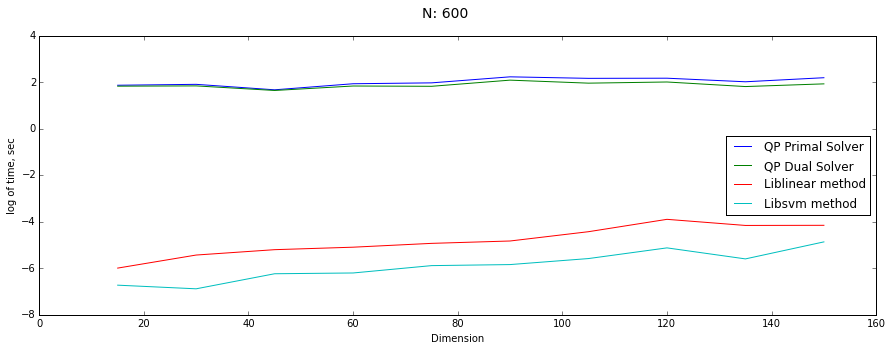
\includegraphics[width=17cm]{1par_N600_one.png}
			\end{center}

			\begin{center}
				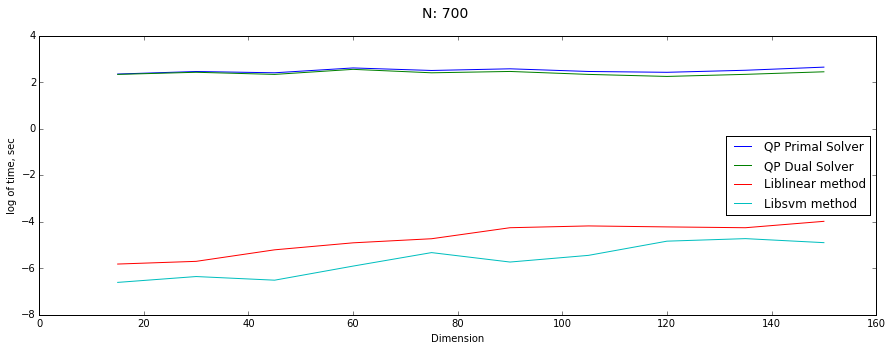
\includegraphics[width=17cm]{1par_N700_one.png}
			\end{center}

			\begin{center}
				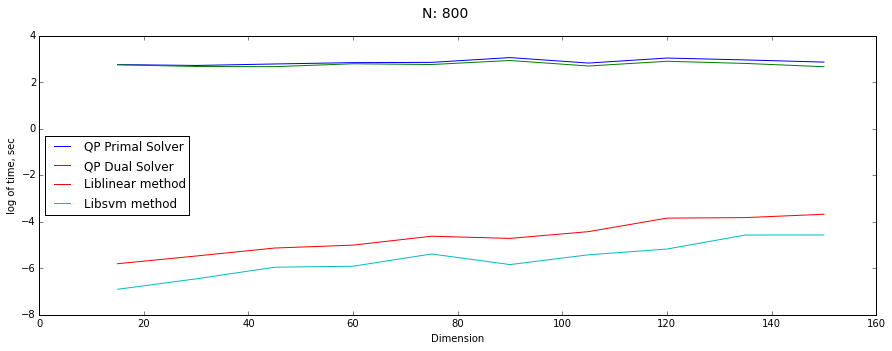
\includegraphics[width=17cm]{1par_N800_one.png}
			\end{center}

			\begin{center}
				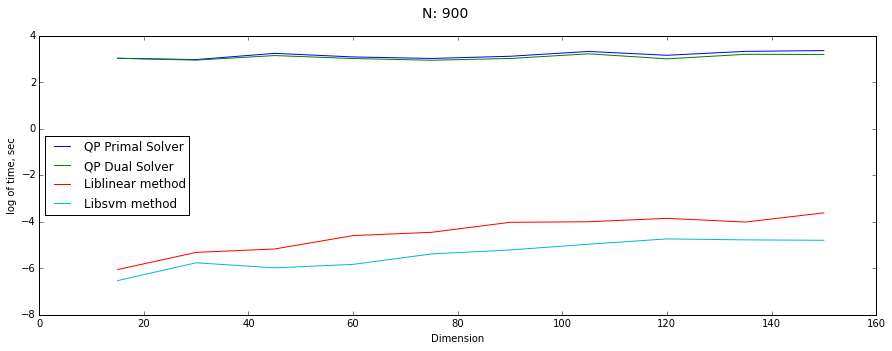
\includegraphics[width=17cm]{1par_N900_one.png}
			\end{center}

			\begin{center}
				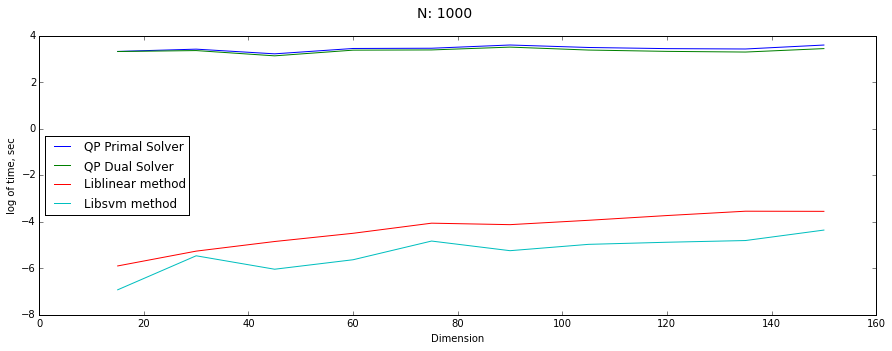
\includegraphics[width=17cm]{1par_N1000_one.png}
			\end{center}

			На следующих графиках представлены значения функционалов в зависимости от размерности пространства в методах с линейным ядром.

			На них можно заметить, что в целом значения для всех методов похожи (одинаковы с некоторой погрешностью).

			\begin{center}
				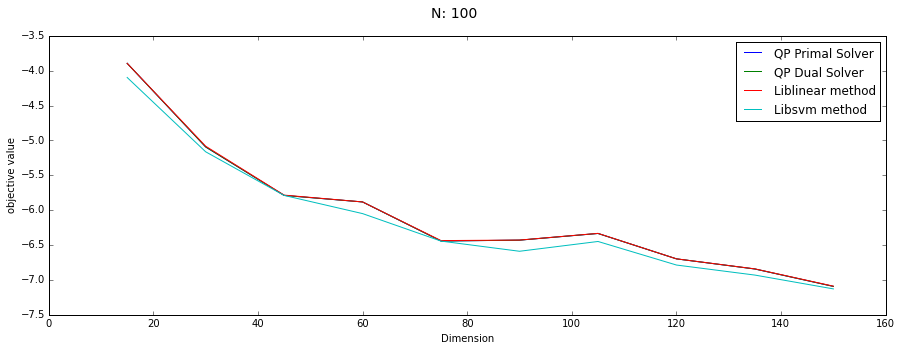
\includegraphics[width=17cm]{1par_obj_N100_one.png}
			\end{center}

			\begin{center}
				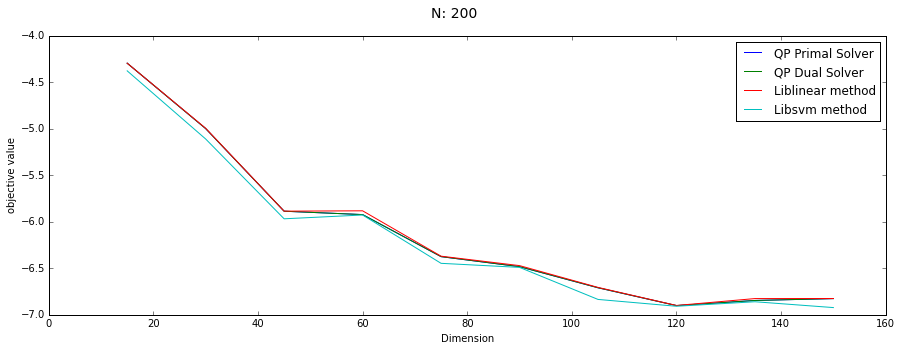
\includegraphics[width=17cm]{1par_obj_N200_one.png}
			\end{center}

			\begin{center}
				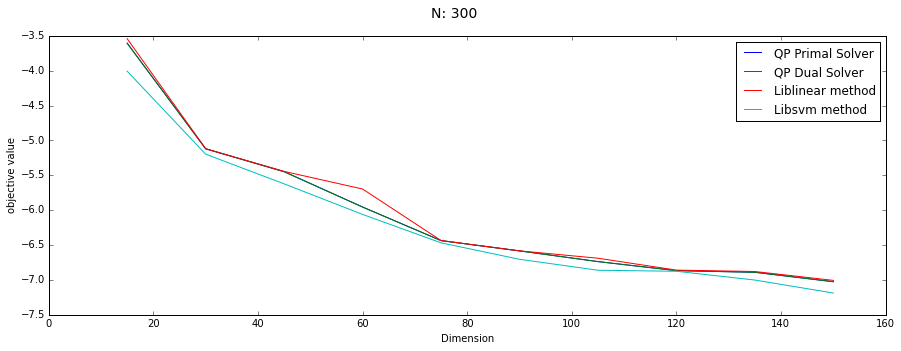
\includegraphics[width=17cm]{1par_obj_N300_one.png}
			\end{center}

			\begin{center}
				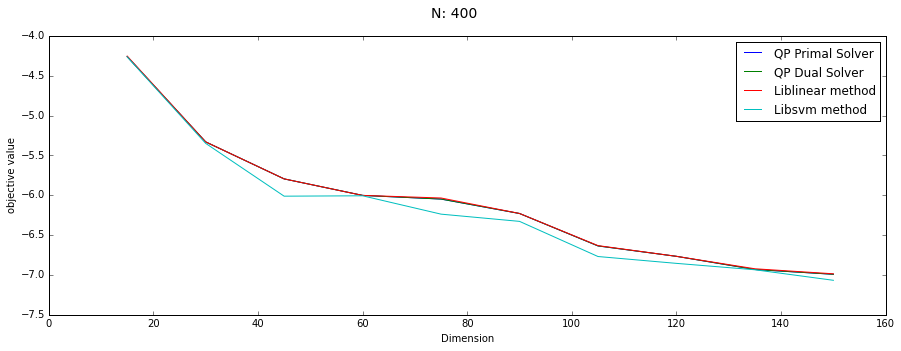
\includegraphics[width=17cm]{1par_obj_N400_one.png}
			\end{center}

			\begin{center}
				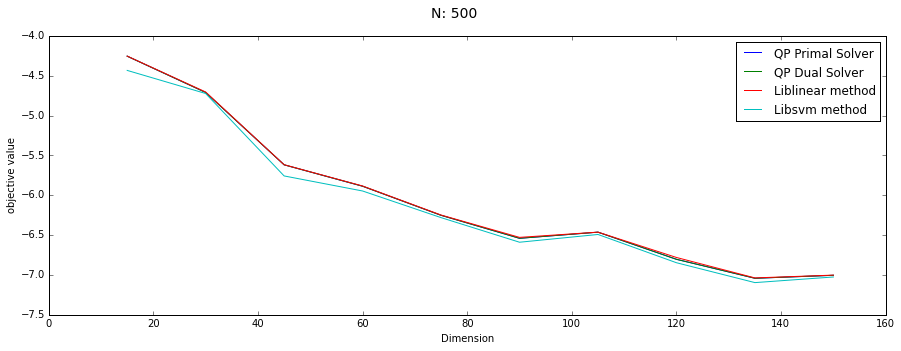
\includegraphics[width=17cm]{1par_obj_N500_one.png}
			\end{center}

			\begin{center}
				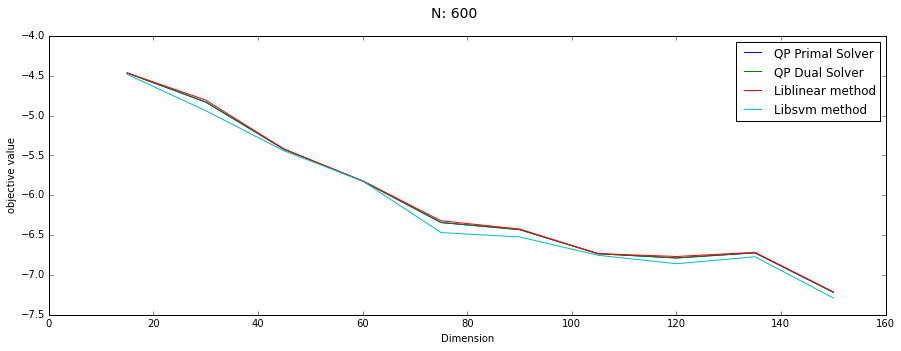
\includegraphics[width=17cm]{1par_obj_N600_one.png}
			\end{center}

			\begin{center}
				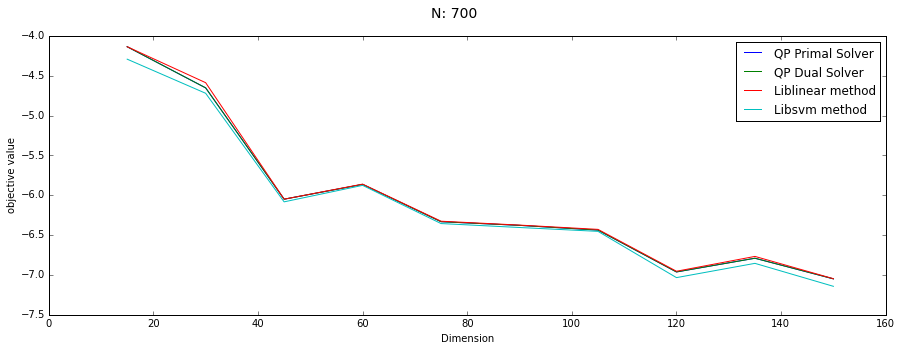
\includegraphics[width=17cm]{1par_obj_N700_one.png}
			\end{center}

			\begin{center}
				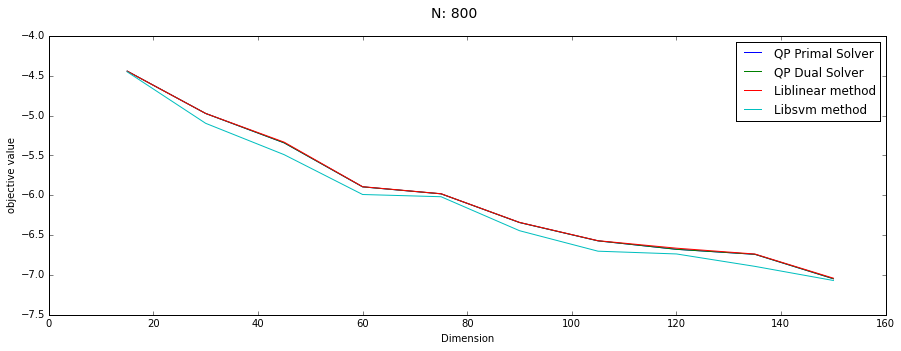
\includegraphics[width=17cm]{1par_obj_N800_one.png}
			\end{center}

			\begin{center}
				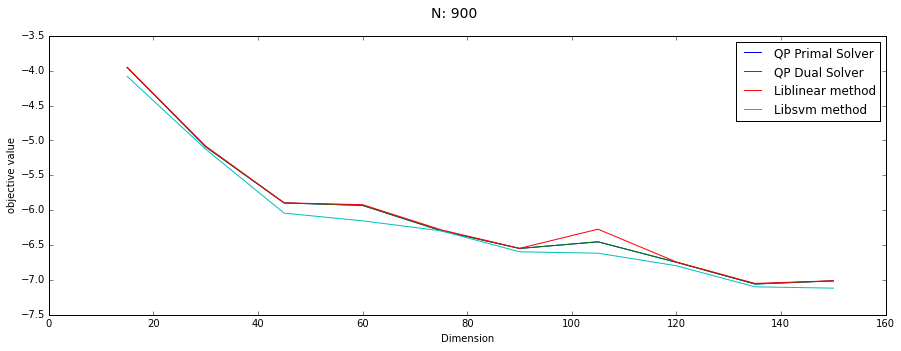
\includegraphics[width=17cm]{1par_obj_N900_one.png}
			\end{center}

			\begin{center}
				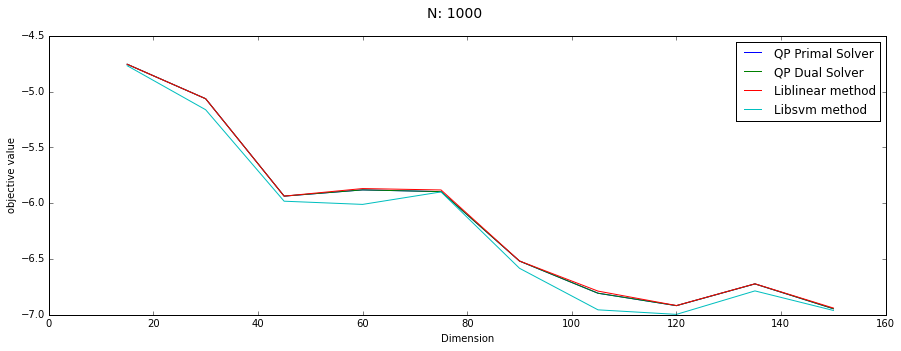
\includegraphics[width=17cm]{1par_obj_N1000_one.png}
			\end{center}

		\newpage
		\subsection{Пункт 2}
			На следующих графиках представлены зависимости времени от размерности пространства для каждого размера выборки в методах с RBF ядром.

			По времени работы быстрым является метод libsvm

			\begin{center}
				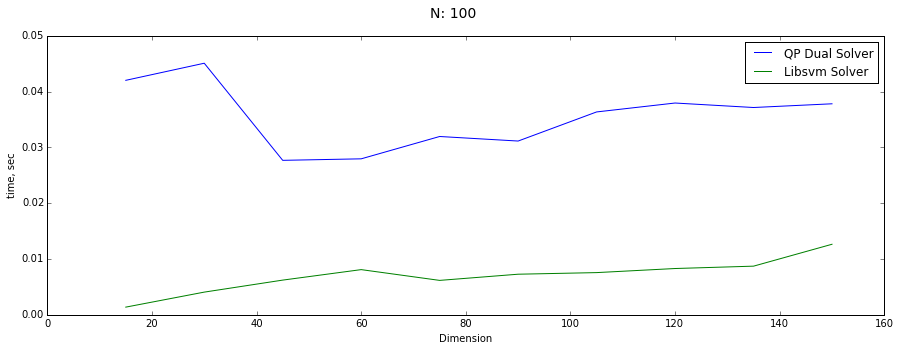
\includegraphics[width=18cm]{2par_N100_one.png}
			\end{center}

			\begin{center}
				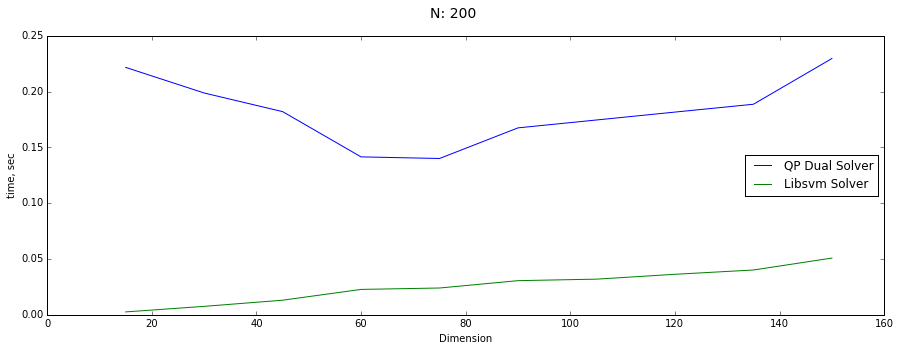
\includegraphics[width=18cm]{2par_N200_one.png}
			\end{center}

			\begin{center}
				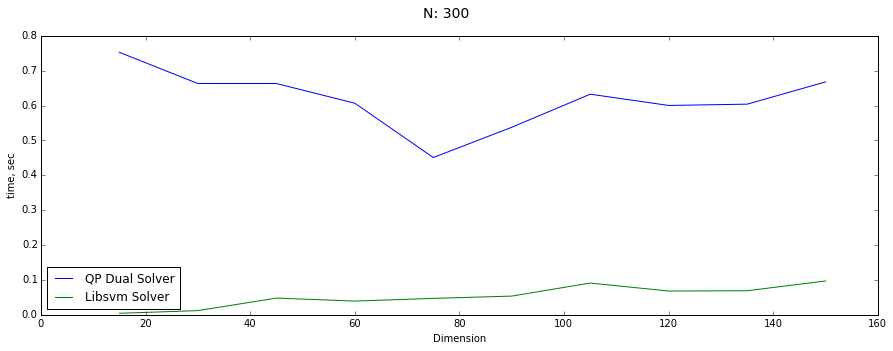
\includegraphics[width=18cm]{2par_N300_one.png}
			\end{center}

			\begin{center}
				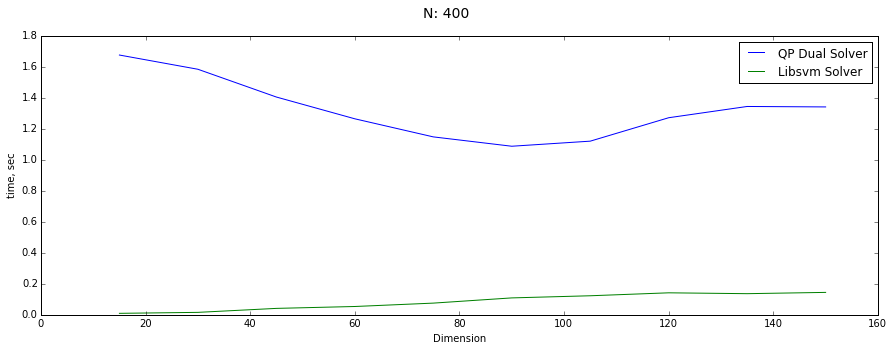
\includegraphics[width=18cm]{2par_N400_one.png}
			\end{center}

			\begin{center}
				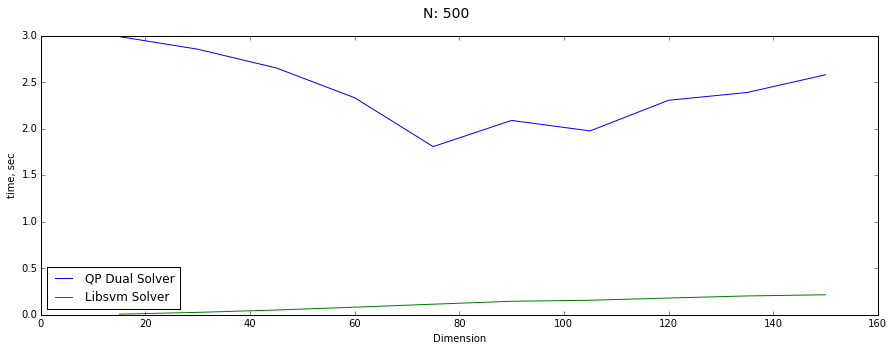
\includegraphics[width=18cm]{2par_N500_one.png}
			\end{center}

			\begin{center}
				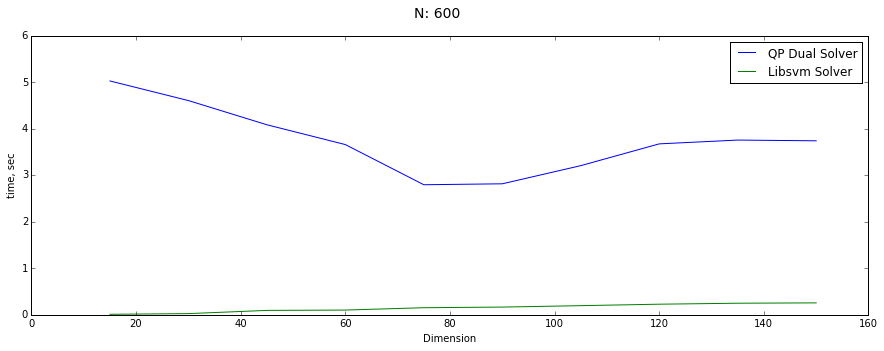
\includegraphics[width=18cm]{2par_N600_one.png}
			\end{center}

			\begin{center}
				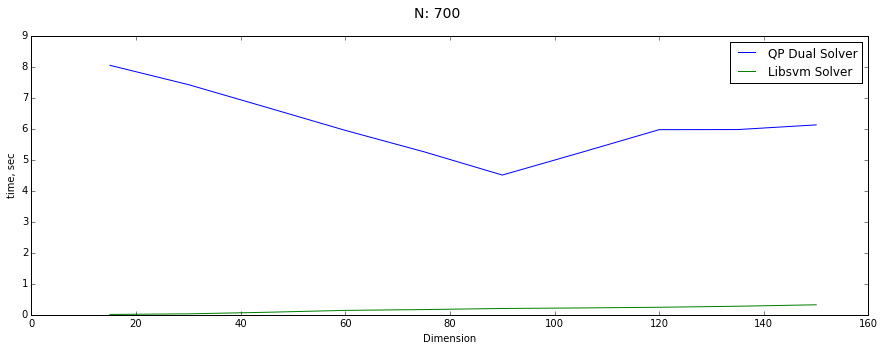
\includegraphics[width=18cm]{2par_N700_one.png}
			\end{center}

			\begin{center}
				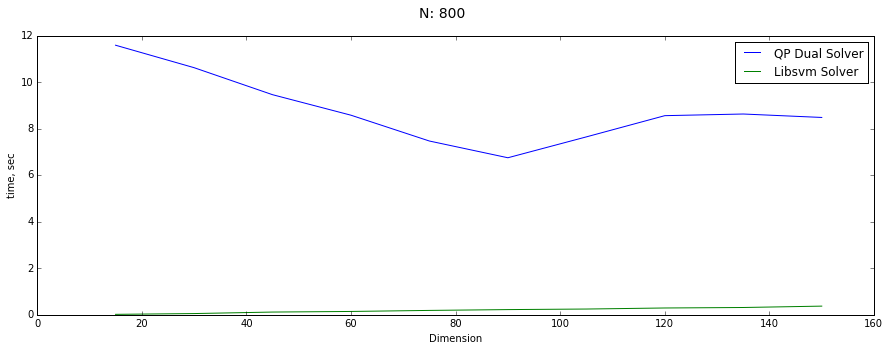
\includegraphics[width=18cm]{2par_N800_one.png}
			\end{center}

			\begin{center}
				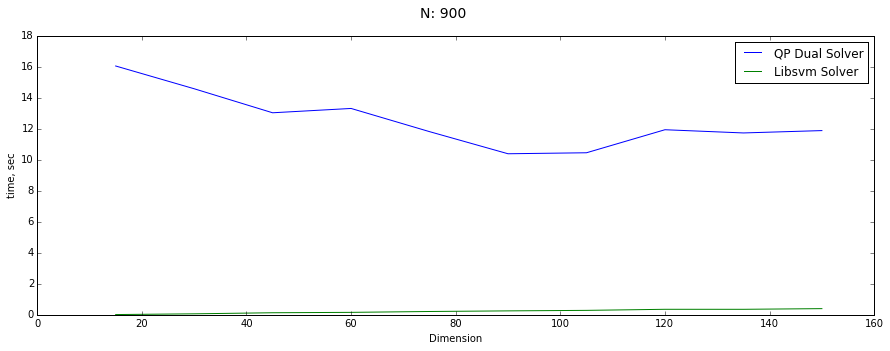
\includegraphics[width=18cm]{2par_N900_one.png}
			\end{center}

			\begin{center}
				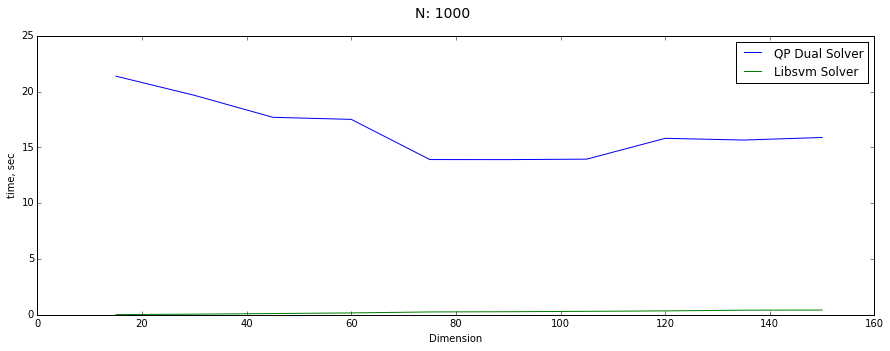
\includegraphics[width=18cm]{2par_N1000_one.png}
			\end{center}

			Далее представлены графики значений функционала для методов с RBF ядром. Для обоих методов они одинаковые с некоторой погрешностью при небольших выборках, но при больших выборках, значения начинают раличаться

			\begin{center}
				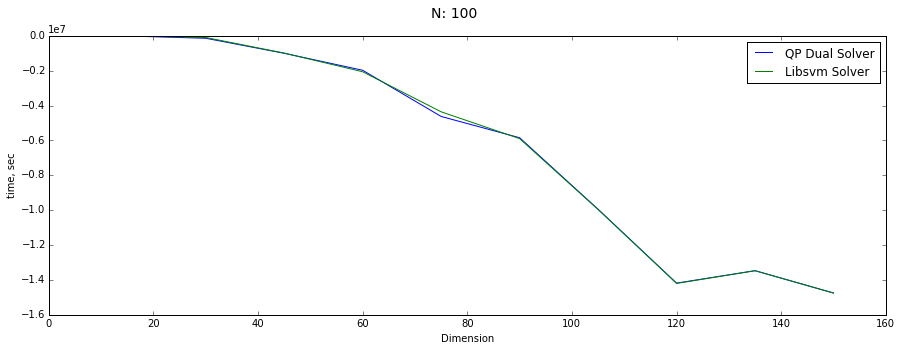
\includegraphics[width=18cm]{2par_obj_N100_one.png}
			\end{center}

			\begin{center}
				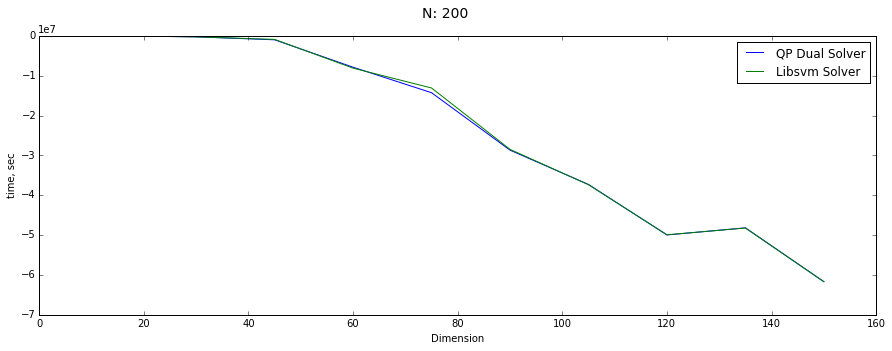
\includegraphics[width=18cm]{2par_obj_N200_one.png}
			\end{center}

			\begin{center}
				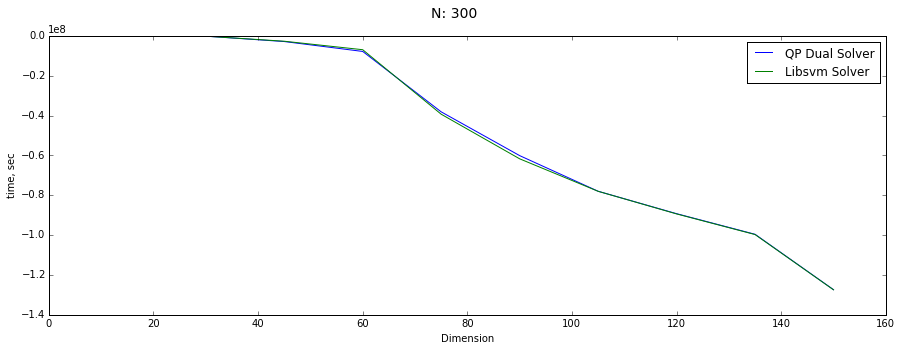
\includegraphics[width=18cm]{2par_obj_N300_one.png}
			\end{center}

			\begin{center}
				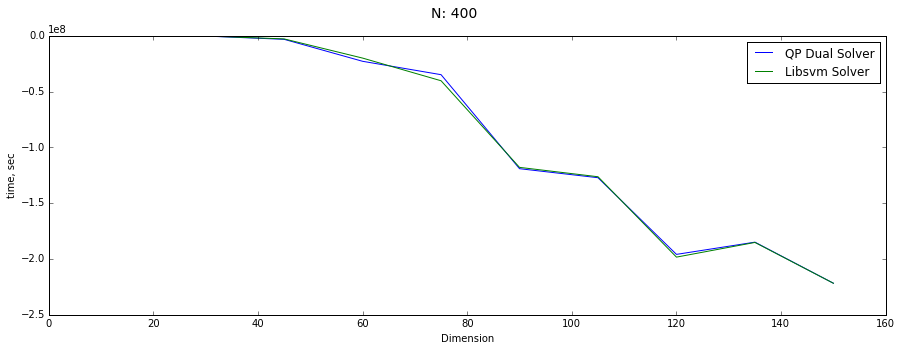
\includegraphics[width=18cm]{2par_obj_N400_one.png}
			\end{center}

			\begin{center}
				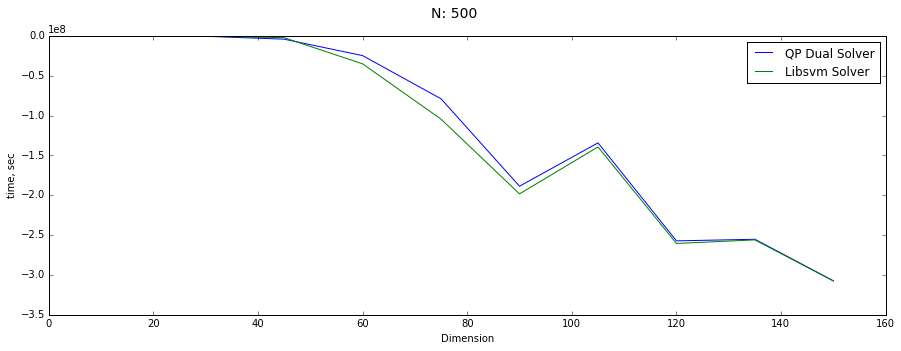
\includegraphics[width=18cm]{2par_obj_N500_one.png}
			\end{center}

			\begin{center}
				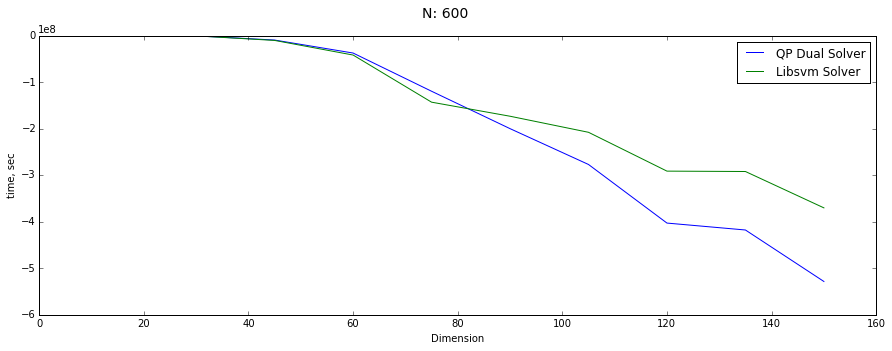
\includegraphics[width=18cm]{2par_obj_N600_one.png}
			\end{center}

			\begin{center}
				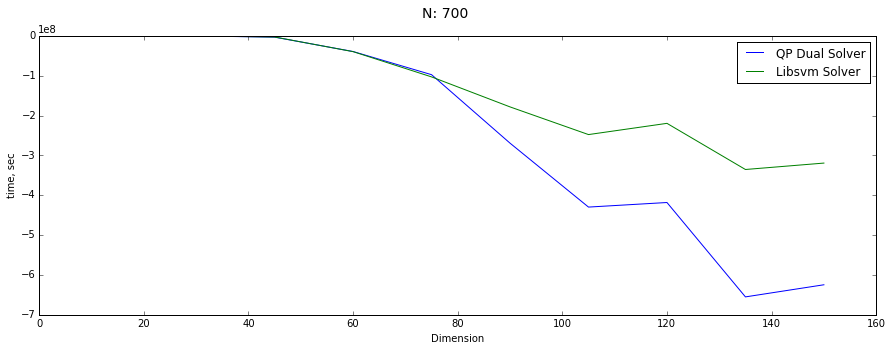
\includegraphics[width=18cm]{2par_obj_N700_one.png}
			\end{center}

			\begin{center}
				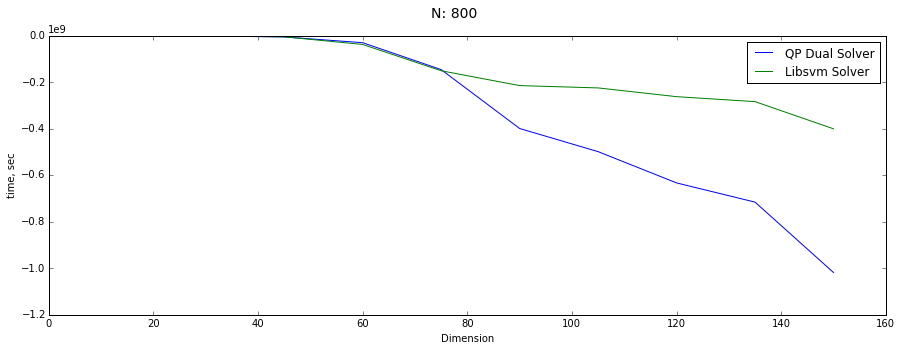
\includegraphics[width=18cm]{2par_obj_N800_one.png}
			\end{center}

			\begin{center}
				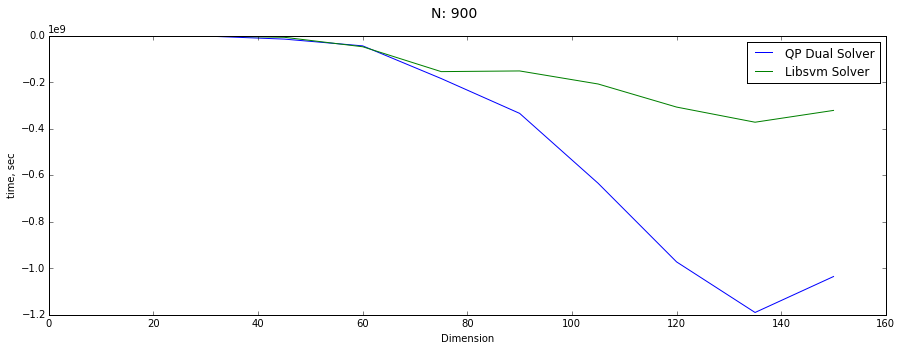
\includegraphics[width=18cm]{2par_obj_N900_one.png}
			\end{center}

			\begin{center}
				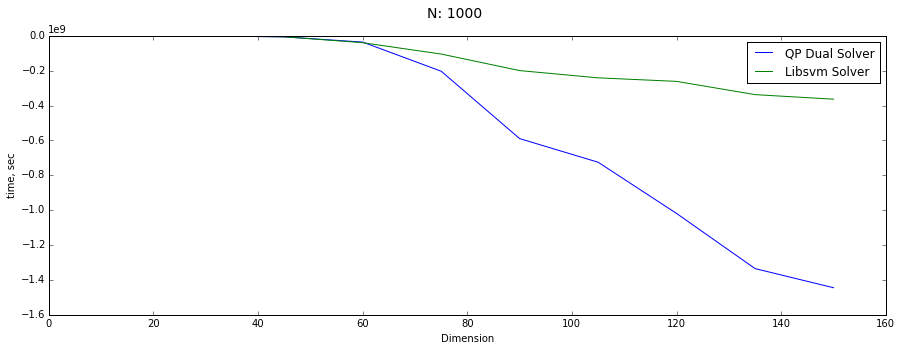
\includegraphics[width=18cm]{2par_obj_N1000_one.png}
			\end{center}

		\newpage
		\subsection{Пункт 3}
			Кросс-валидация реализована с помощью библиотеки sklearn на методе libsvm.

			Исследуем точность классификации в зависимости от параметра C

			\begin{center}{\bf Плохо разделимая выборка}\end{center}

			\begin{center}
			\begin{tabular}{c c}
				Линейное ядро & RBF ядро \\
				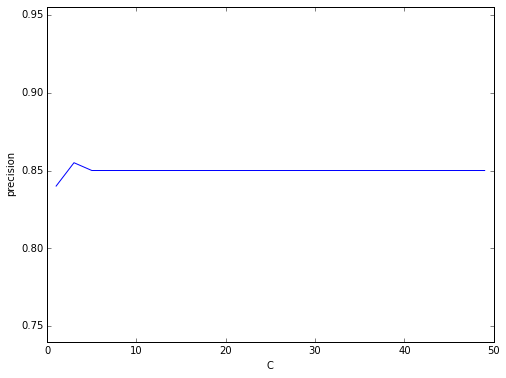
\includegraphics[width=8cm]{3par_bad_lin_C.png} &
				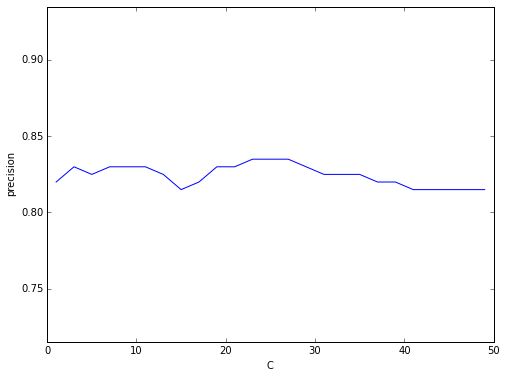
\includegraphics[width=8cm]{3par_bad_rbf_C.png}
			\end{tabular}				
			\end{center}

			\begin{center}{\bf Хорошо разделимая выборка}\end{center}

			\begin{center}
			\begin{tabular}{c c}
				Линейное ядро & RBF ядро \\
				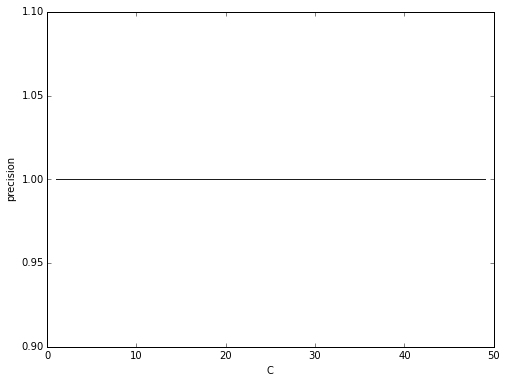
\includegraphics[width=8cm]{3par_good_lin_C.png} &
				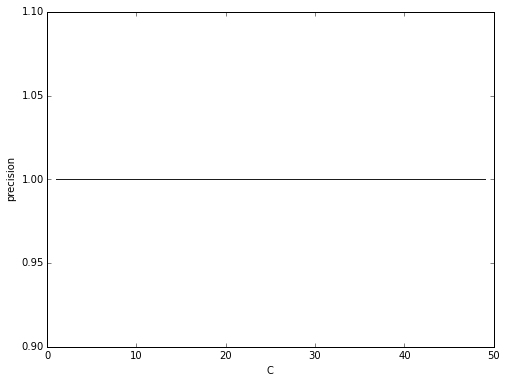
\includegraphics[width=8cm]{3par_good_rbf_C.png}
			\end{tabular}				
			\end{center}


			Исследуем точность классификации в зависимости от параметра $\gamma$

			\begin{center}
			\begin{tabular}{c c}
				Плохо разделимая выборка & Хорошо разделимая выборка \\
				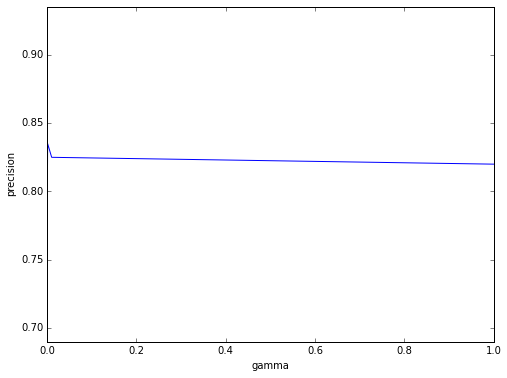
\includegraphics[width=8cm]{3par_bad_rbf_gamma.png} &
				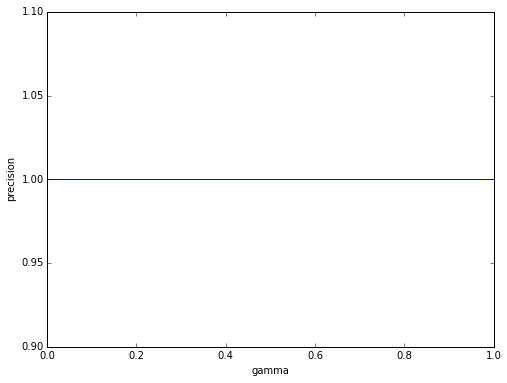
\includegraphics[width=8cm]{3par_good_rbf_gamma.png}
			\end{tabular}
			\end{center}

			В плохо разделимой выборке видим, что максимальная точность в случае лмнейного ядра достигается при C = 3, а в случае RBF ядра максимум достигается при C = 25. А точность в зависимости от $\gamma$ убывает. Т.е. классификатор более точен при гамма близком к нулю.

			В хорошо разделимой выборке для любого C и в случае линейного ядра, и в случае RBF ядра, точность остается постоянной и равной 1. А точность от гамма также не зависит.



		\newpage
		\subsection{Пункт 4}
			На следующих графиках показаны зависимости времени работы и значений функционала от $\beta$ при разных $\alpha$ для метода субградиентного спуска.
			По ним можно сделать вывод, что при $\beta = 1$ и $\alpha = 2$ метод работает сравнительно медлоенно, но выдает более точное значение функционала

			\begin{center}
				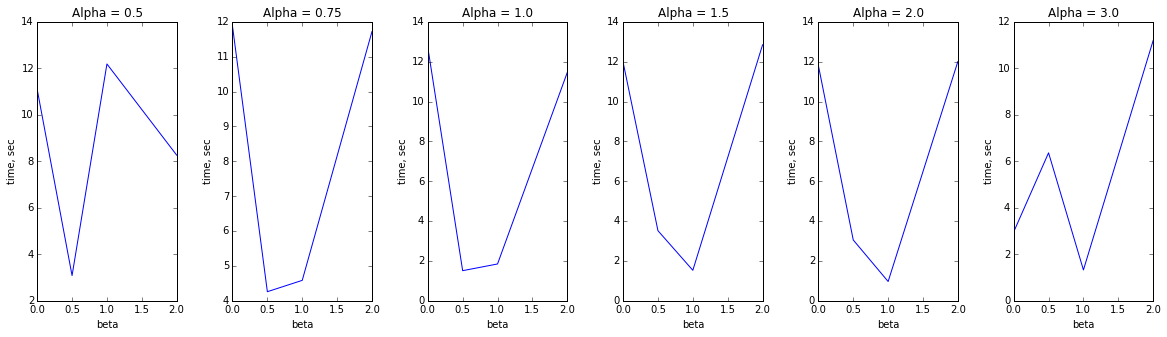
\includegraphics[width=18cm]{4par.png}
			\end{center}

			\begin{center}
				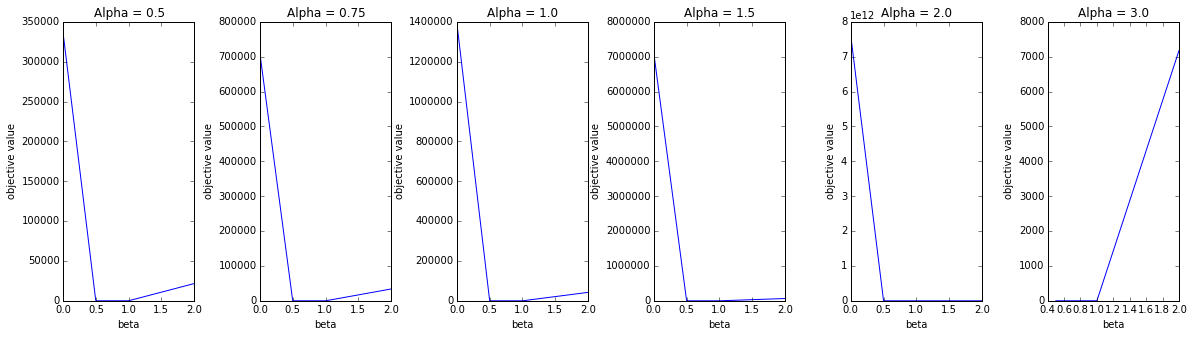
\includegraphics[width=18cm]{4par_obj.png}
			\end{center}

			Далее приведем графики сходимости субградиентного спуска при разных значения $\alpha$ и $\beta$

			\begin{center}
				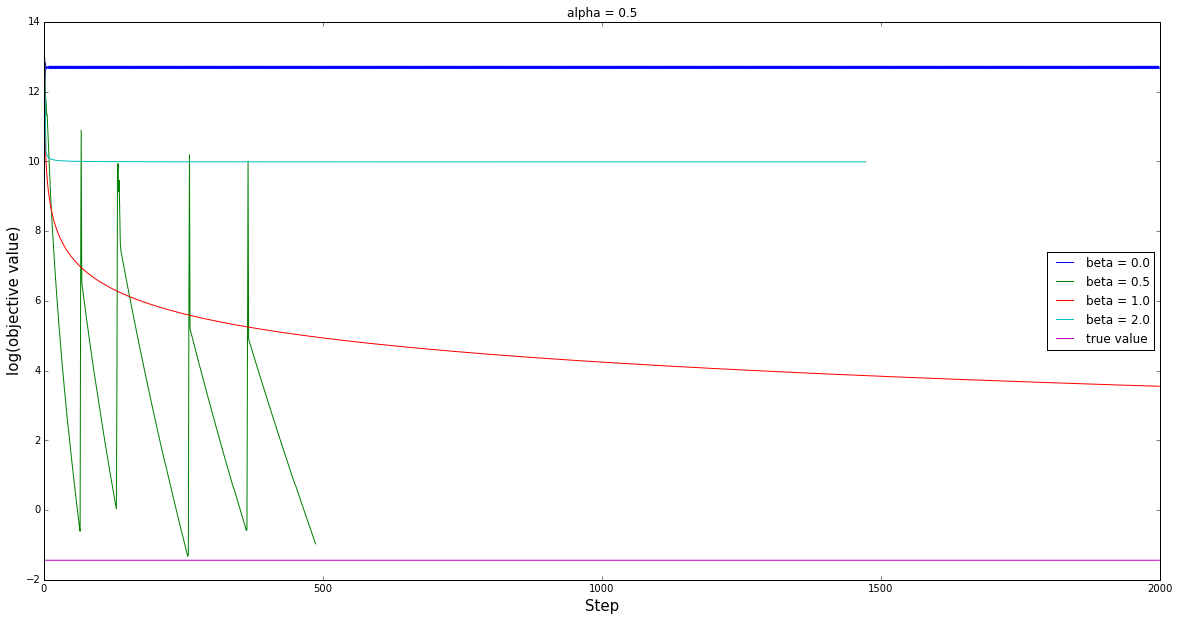
\includegraphics[width=16cm]{4par_05.png}
			\end{center}

			\begin{center}
				\includegraphics[width=16cm]{4par_075.png}
			\end{center}

			\begin{center}
				\includegraphics[width=16cm]{4par_10.png}
			\end{center}

			\begin{center}
				\includegraphics[width=16cm]{4par_15.png}
			\end{center}

			\begin{center}
				\includegraphics[width=16cm]{4par_20.png}
			\end{center}

			\begin{center}
				\includegraphics[width=16cm]{4par_30.png}
			\end{center}

			Из этих графиков тоже видно, что метод сходится быстро при $\beta = 1$ и $\alpha = 2$ 

		\newpage
		\subsection{Пункт 5}
			На следующих графиках показаны зависимости времени работы и значений функционала от доли размера подвыборки в методе стохастического субградиентного спуска.
			На них видно, что более близкое к реальному значение функционала получается при размере 90\% от размера выборки. Время работы сравнительно среднее при данном размере подвыборки.

			\begin{center}
				\includegraphics[width=18cm]{5par.png}
			\end{center}

			На следующем графике показаны скорости сходимости метода в зависимости от доли размера подвыборки

			\begin{center}
				\includegraphics[width=18cm]{5par_one.png}
			\end{center}

			Из него также видно, что близкое к реальному значение функционала получается при 90\% от размера выборки, а также видно, что при этом значении размера, метод сходится за меньшее число шагов.

		\newpage
		\subsection{Пункт 6}
			Сравним методы OneVsOne и OneVsAll

			На первом графике представлен метод OneVsAll на примере liblinear. Видно, что разделяющие поверхности не точно разделяют выборки между собой, хотя данная выборка является линейно разделимой
			\begin{center}
				\includegraphics[width=15cm]{6par.png}
			\end{center}

			На следующем графике видно, что классификатор сработал хорошо. В данном графике представлен метод OneVsOne на примере libsvm
			\begin{center}
				\includegraphics[width=15cm]{6par_dual.png}
			\end{center}

			Далее представлен метод OneVsOne на примере libsvm с rbf ядром 0.01
			\begin{center}
				\includegraphics[width=15cm]{6par_rbf1.png}
			\end{center}

			На этом графике представлен метод OneVsOne на примере libsvm с rbf ядром 1
			\begin{center}
				\includegraphics[width=15cm]{6par_rbf2.png}
			\end{center}

		\newpage
		\subsection{Пункт 7}
			Метод субградиентного спуска
			\begin{center}
				\includegraphics[width=16cm]{7par_grad.png}
			\end{center}

			Метод стохастического субградиентного спуска
			\begin{center}
				\includegraphics[width=16cm]{7par_st_grad.png}
			\end{center}

			~\newline
			
			Метод primal solver
			\begin{center}
				\includegraphics[width=16cm]{7par_primal.png}
			\end{center}

			Метод dual solver
			\begin{center}
				\includegraphics[width=16cm]{7par_dual.png}
			\end{center}
			
			~\newline
			~\newline
			
			Метод primal solver с rbf ядром
			\begin{center}
				\includegraphics[width=16cm]{7par_dual_rbf.png}
			\end{center}

			Метод liblinear
			\begin{center}
				\includegraphics[width=16cm]{7par_liblin.png}
			\end{center}

			~\newline
			~\newline

			Метод libsvm
			\begin{center}
				\includegraphics[width=16cm]{7par_libsvm.png}
			\end{center}

			Метод libsvm с rbf ядром
			\begin{center}
				\includegraphics[width=16cm]{7par_libsvm_rbf.png}
			\end{center}

		\newpage
		\subsection{Пункт 8}
			Для тестирования MNIST использовалась подвыборка из 200 элементов на каждый класс и метод OneVsOne. Выборка генерировалась случайным образом: данные для обучения выбирались из первых 60000 объектов (встроенная разбивка на обучение-контроль), а данные для тестирования выбирались из последних 10000 объектов. При этом количество объектов каждого класса одинаковые (в данном случае по 200 объектов)

			\begin{center}
			\begin{tabular}{| l | l | l |}
				\hline
				Метод & Время работы & Точность \\
				\hline
				Primal solver & 48.5 сек & 0.90749 \\
				\hline
				Dual solver & 5.7 сек & 0.90600 \\
				\hline
				Dual solver с rbf ядром & 5.15 сек & 0.81299 \\
				\hline
				Liblinear & 0.616 сек & 0.90749 \\
				\hline
				Libsvm & 1.52 сек & 0.90649 \\
				\hline
				Libsvm с rbf ядром & 8.92 сек & 0.76500 \\
				\hline
			\end{tabular}
			\end{center}

			По этим данным можно сделать вывод, что самый быстрый и самый точный метод для классификации MNIST - это метод liblinear

	\newpage
	\section{Заключение}
		По результатам исследований выяснилось, что каждый метод решения одного и того же задания работает не похоже друг на друга. У каждого метода разное время работы и разные точности и для каждой задачи нужно выбирать метод с умом. В нашем случае, тесты показали, что для классификации MNIST надо выбирать метод liblinear решения задачи SVM.

		P.S. Для полного MNIST я не смог дождаться завершения обучения на liblinear (слабый процессор), но оставил код, чтобы попробовали запустить MNIST у себя на компьютере.

	\newpage
	\section{Приложение}
		\subsection{Отдельные графики 1-го пункта}
			Исследуем зависимость времени работы методов от размерности пространства для каждого размера выборки.
			
			На слелующих фото представлены графики зависимости времени работы от размерности пространства. На них можно увидеть, что самый быстрый метод libsvm, далее liblinear

			\begin{center}
				\includegraphics[width=18cm]{1par_N100.png}
			\end{center}

			\begin{center}
				\includegraphics[width=18cm]{1par_N200.png}
			\end{center}

			\begin{center}
				\includegraphics[width=18cm]{1par_N300.png}
			\end{center}

			\begin{center}
				\includegraphics[width=18cm]{1par_N400.png}
			\end{center}

			\begin{center}
				\includegraphics[width=18cm]{1par_N500.png}
			\end{center}

			\begin{center}
				\includegraphics[width=18cm]{1par_N600.png}
			\end{center}

			\begin{center}
				\includegraphics[width=18cm]{1par_N700.png}
			\end{center}

			\begin{center}
				\includegraphics[width=18cm]{1par_N800.png}
			\end{center}

			\begin{center}
				\includegraphics[width=18cm]{1par_N900.png}
			\end{center}

			\begin{center}
				\includegraphics[width=18cm]{1par_N1000.png}
			\end{center}

			На следующих графиках представлены значения функционалов в зависимости от размерности пространства.

			На них можно заметить, что значения одинаковые для методов primal и liblinear, а также для методов dual и libsvm. В целом значения для всех методов похожи.

			\begin{center}
				\includegraphics[width=18cm]{1par_obj_N100.png}
			\end{center}

			\begin{center}
				\includegraphics[width=18cm]{1par_obj_N200.png}
			\end{center}

			\begin{center}
				\includegraphics[width=18cm]{1par_obj_N300.png}
			\end{center}

			\begin{center}
				\includegraphics[width=18cm]{1par_obj_N400.png}
			\end{center}

			\begin{center}
				\includegraphics[width=18cm]{1par_obj_N500.png}
			\end{center}

			\begin{center}
				\includegraphics[width=18cm]{1par_obj_N600.png}
			\end{center}

			\begin{center}
				\includegraphics[width=18cm]{1par_obj_N700.png}
			\end{center}

			\begin{center}
				\includegraphics[width=18cm]{1par_obj_N800.png}
			\end{center}

			\begin{center}
				\includegraphics[width=18cm]{1par_obj_N900.png}
			\end{center}

			\begin{center}
				\includegraphics[width=18cm]{1par_obj_N1000.png}
			\end{center}

		\newpage
		\subsection{Отдельные графики 2-го пункта}
			На следующих графиках представлены зависимости времени от размерности пространства для каждого размера выборки.

			По времени работы быстрым является метод libsvm

			\begin{center}
				\includegraphics[width=18cm]{2par_N100.png}
			\end{center}

			\begin{center}
				\includegraphics[width=18cm]{2par_N200.png}
			\end{center}

			\begin{center}
				\includegraphics[width=18cm]{2par_N300.png}
			\end{center}

			\begin{center}
				\includegraphics[width=18cm]{2par_N400.png}
			\end{center}

			\begin{center}
				\includegraphics[width=18cm]{2par_N500.png}
			\end{center}

			\begin{center}
				\includegraphics[width=18cm]{2par_N600.png}
			\end{center}

			\begin{center}
				\includegraphics[width=18cm]{2par_N700.png}
			\end{center}

			\begin{center}
				\includegraphics[width=18cm]{2par_N800.png}
			\end{center}

			\begin{center}
				\includegraphics[width=18cm]{2par_N900.png}
			\end{center}

			\begin{center}
				\includegraphics[width=18cm]{2par_N1000.png}
			\end{center}

			Далее представлены графики значений функционала. Для обоих методов они одинаковые

			\begin{center}
				\includegraphics[width=18cm]{2par_obj_N100.png}
			\end{center}

			\begin{center}
				\includegraphics[width=18cm]{2par_obj_N200.png}
			\end{center}

			\begin{center}
				\includegraphics[width=18cm]{2par_obj_N300.png}
			\end{center}

			\begin{center}
				\includegraphics[width=18cm]{2par_obj_N400.png}
			\end{center}

			\begin{center}
				\includegraphics[width=18cm]{2par_obj_N500.png}
			\end{center}

			\begin{center}
				\includegraphics[width=18cm]{2par_obj_N600.png}
			\end{center}

			\begin{center}
				\includegraphics[width=18cm]{2par_obj_N700.png}
			\end{center}

			\begin{center}
				\includegraphics[width=18cm]{2par_obj_N800.png}
			\end{center}

			\begin{center}
				\includegraphics[width=18cm]{2par_obj_N900.png}
			\end{center}

			\begin{center}
				\includegraphics[width=18cm]{2par_obj_N1000.png}
			\end{center}

\end{document}
